\section{Enterprise Integration Patterns (EIP)}
Integration patterns are a set of design patterns that can be used to solve common integration problems when connecting different systems and applications. These patterns provide a common language and best practices for designing and implementing integration solutions. It is a "known use" of Pipes \& Filters Pattern (Patterns of Software Architecture, Volume 1).

In essence, a message is transmitted in five steps:
\begin{description}
  \item[Create] the sender creates the message and populates it with data.
  \item[Send] the sender adds the message to a channel.
  \item[Deliver] the messaging system moves the message from the sender’s computer to the receiver’s computer, making it available to the receiver.
  \item[Receive] the receiver reads the message from the channel.
  \item[Process ] the receiver extracts the data from the message.
\end{description}

\subsection{Integration Styles}
\subsubsection{File Transfer}
\begin{minipage}{.4\textwidth}
  \begin{figure}[H]
    \center
    \caption{Shared Database}
    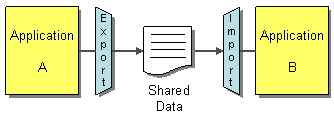
\includegraphics[width=\textwidth]{filetransfer}
    \caption{File Transfer}
  \end{figure}
\end{minipage}
\begin{minipage}[b]{.6\textwidth}
  Have each application produce files containing information that other applications need to consume. Integrators take the responsibility of transforming files into different formats. Produce the files at regular intervals according to the nature of the business.
\end{minipage}

\subsubsection{Shared Database}
\begin{minipage}{.4\textwidth}
  \begin{figure}[H]
    \center
    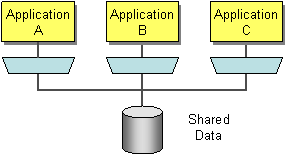
\includegraphics[width=\textwidth]{shareddatabase}
    \caption{Shared Database}
  \end{figure}
\end{minipage}
\begin{minipage}[b]{.6\textwidth}
  Integrate applications by having them store their data in a single Shared Database.
\end{minipage}

\subsubsection{Remote Procedure Call}
\begin{minipage}{.4\textwidth}
  \begin{figure}[H]
    \center
    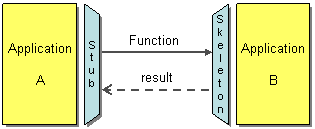
\includegraphics[width=0.75\textwidth]{rpc}
    \caption{Remote Procedure Call}
  \end{figure}
\end{minipage}
\begin{minipage}[b]{.6\textwidth}
  Develop each application as a large-scale object or component with encapsulated data. Provide an interface to allow other applications to interact with the running application.
\end{minipage}

\subsubsection{Messaging}
\begin{minipage}{.4\textwidth}
  \begin{figure}[H]
    \center
    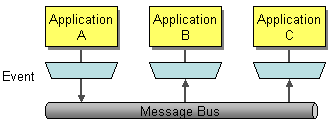
\includegraphics[width=\textwidth]{integrationstyle-messaging}
    \caption{Messaging}
  \end{figure}
\end{minipage}
\begin{minipage}[b]{.6\textwidth}
  Use Messaging to transfer packets of data frequently, immediately, reliably, and asynchronously, using customizable formats.
\end{minipage}

\subsection{Asynchronous Messaging}
Messaging capabilities are typically provided by a separate software system called a messaging system or message-oriented middleware (MOM), which is comparable to database systems that manage data persistence.

\begin{itemize}
  \item Database administrator populates database with schema for application data; MOM administrator configures the messaging system with channels that define the paths of communication between the applications. Messaging system manages sending and receiving of messages.
  \item Database makes sure each data record is safely persisted, and likewise main task of messaging system is to move messages from the sender’s computer to the receiver’s computer in a reliable fashion.
\end{itemize}

The reason a messaging system is needed to move messages from one computer to another is that computers and the networks that connect them are inherently unreliable. Just because one application is ready to send a communication does not mean that the other application is ready to receive it. Even if both applications are ready, the network may not be working, or may fail to transmit the data properly. A messaging system overcomes these limitations by repeatedly trying to transmit the message until it succeeds. Under ideal circumstances, the message is transmitted successfully on the first try, but circumstances are often not ideal.

\paragraph{Loose coupling dimensions:}
\begin{description}
  \item [Reference Autonomy] Producers and Consumers don't know each other
  \item [Platform Autonomy] Producers and consumers may be located in different technical environment (e.g. containers), can be written in different languages.
  \item [Time Autonomy] Producers and Consumers access channel at their own pace: Communication is asynchronous, Data exchanged is persistent
  \item [Format Autonomy] Producers and consumers may use different formats of exchanged Data
\end{description}

\begin{figure}[H]
  \center
  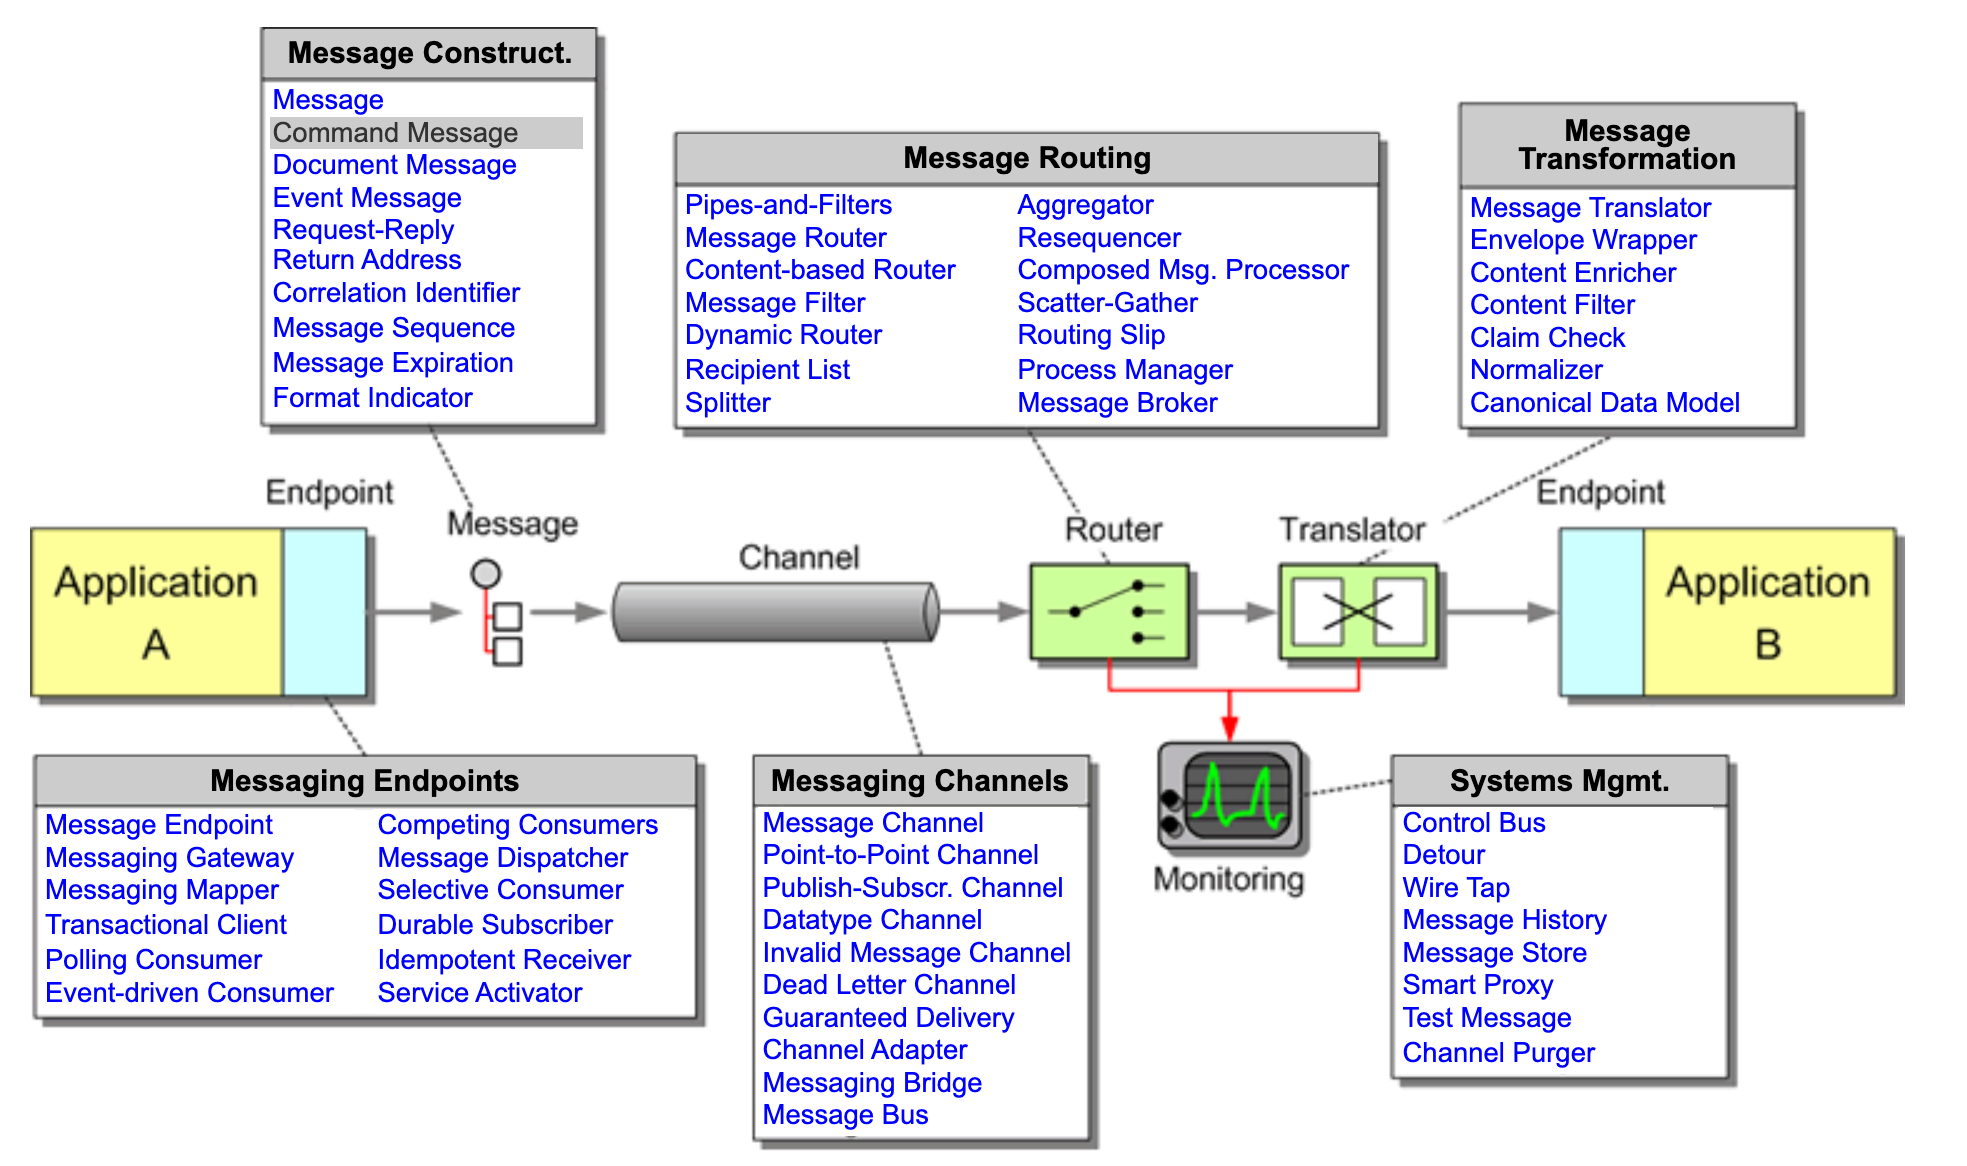
\includegraphics[width=0.9\textwidth]{messaging}
  \caption{EIP Pattern Categories}
\end{figure}

\pagebreak

\subsection{Message Construction Patterns}
Describes the intent, form and content of the messages that travel across the messaging system.

\subsubsection{Document Message Pattern}
Use a Document Message to reliably transfer data structure between applications. Whereas a Command Message tells the receiver to invoke certain behavior, a Document Message just passes data and lets the receiver decide what, if anything, to do with the data. The data is a single unit of data, a single object or data structure which may decompose into smaller units.

\begin{figure}[H]
  \center
  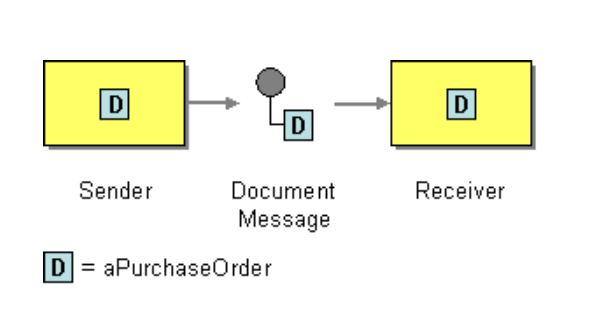
\includegraphics[width=0.5\textwidth]{documentmessage}
  \caption{Document Message}
\end{figure}

\subsubsection{Command Message Pattern}
Use a Command Message to reliably invoke a procedure in another application. There is no specific message type for commands; a Command Message is simply a regular message that happens to contain a command. In JMS, the command message could be any type of message; examples include an ObjectMessage containing a Serializable command object, a TextMessage containing the command in XML form, etc.

\begin{figure}[H]
  \center
  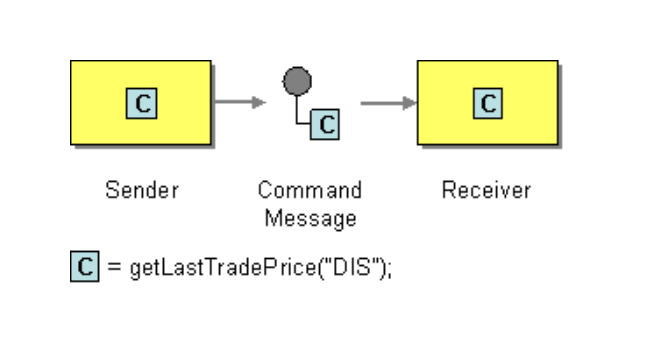
\includegraphics[width=0.5\textwidth]{commandmessagepattern}
  \caption{Command Message Pattern}
\end{figure}

\subsubsection{Message Expiration}
The Message Expiration can be used to specify a time limit, how long the message is viable. Once the time for which a message is viable passes, and the message still has not been consumed, then the message will expire. The messaging system’s consumers will ignore an expired message; they treat the message as if it where never sent in the first place. Most messaging system implementations reroute expired messages to the Dead Letter Channel, while others simply discard expired messages; this may be configurable.

\begin{figure}[H]
  \center
  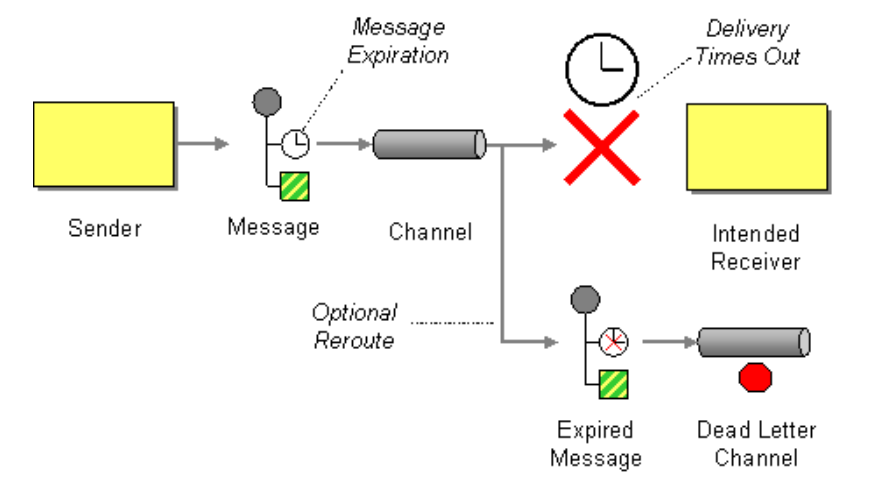
\includegraphics[width=0.65\textwidth]{messageexpiration}
  \caption{Message Expiration}
\end{figure}

\subsubsection{Request-Reply Pattern}
When an application sends a message, how can it get a response from the receiver? Send a pair of Request-Reply messages, each on its own channel. The request message should contain a Return Address that indicates where to send the reply message.

\begin{figure}[H]
  \center
  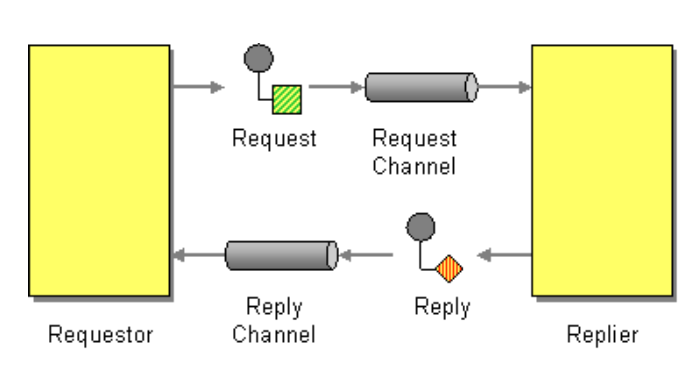
\includegraphics[width=0.5\textwidth]{requestreplypattern}
  \caption{Request-Reply Pattern}
\end{figure}

\pagebreak

\subsection{Messaging Channels}

\subsubsection{Point-to-Point Channel}
Send the message on a Point-to-Point Channel, which ensures that only one receiver will receive a particular message. Ensures that only one receiver consumes any given message. If the channel has multiple receivers, only one of them can successfully consume a particular message. If multiple receivers try to consume a single message, the channel ensures that only one of them succeeds, so the receivers do not have to coordinate with each other. The channel can still have multiple receivers to consume multiple messages concurrently, but only a single receiver consumes any one message.

\begin{figure}[h!]
  \center
  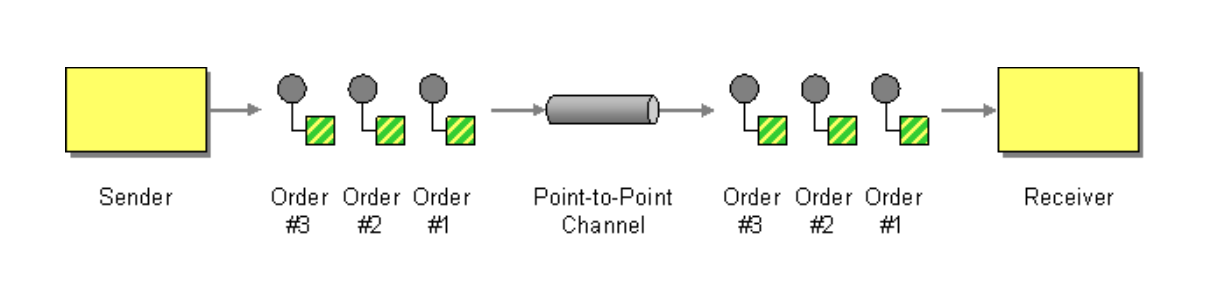
\includegraphics[width=0.9\textwidth]{pointtopointmessaging}
  \caption{Point-to-Point Messaging}
\end{figure}

\subsubsection{Publish-Subscribe Channel}
Send the event on a Publish-Subscribe Channel, which delivers a copy of a particular event to each receiver. Has one input channel that splits into multiple output channels, one for each subscriber. When an event is published into the channel, the Publish-Subscribe Channel delivers a copy of the message to each of the output channels. Each output channel has only one subscriber, which is only allowed to consume a message once. Each subscriber only gets the message once and consumed copies disappear from their channels.

\begin{figure}[H]
  \center
  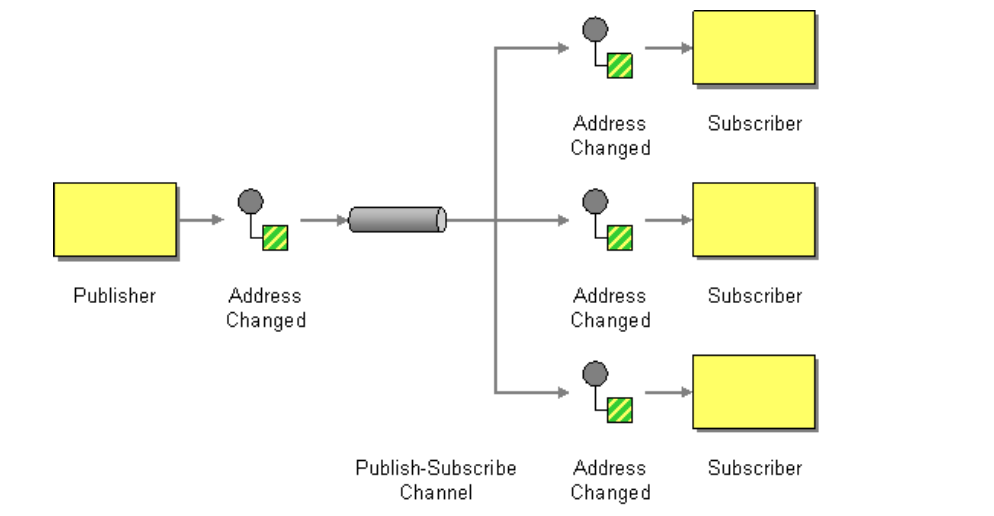
\includegraphics[width=0.75\textwidth]{publishandsubscribe}
  \caption{Publish-Subscribe Channel}
\end{figure}

\subsubsection{Guaranteed Delivery Pattern}
Use Guaranteed Delivery to make messages persistent so that they are not lost even if the messaging system crashes.  With Guaranteed Delivery, the messaging system uses a built-in data store to persist messages. Each computer the messaging system is installed on has its own data store so that the messages can be stored locally. When the sender sends a message, the send operation does not complete successfully until the message is safely stored in the sender’s data store. Subsequently, the message is not deleted from one data store until it is successfully forwarded to and stored in the next data store.

\begin{figure}[H]
  \center
  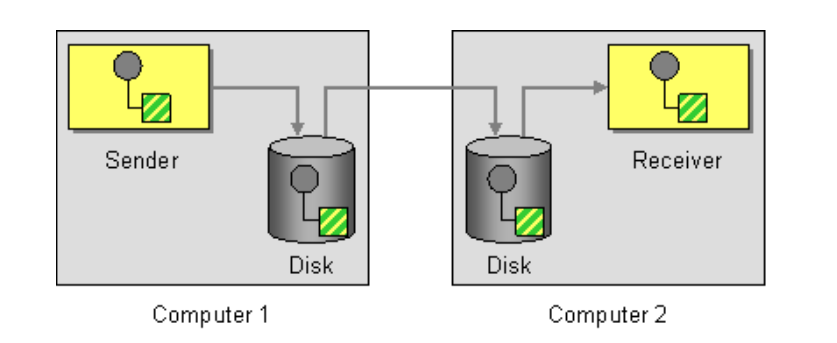
\includegraphics[width=0.5\textwidth]{guaranteeddelivery}
  \caption{Guaranteed Delivery Pattern}
\end{figure}

\subsubsection{Dead Letter Channel Pattern}
When a messaging system determines that it cannot or should not deliver a message, it may elect to move the message to a Dead Letter Channel. The specific way a Dead Letter Channel works depends on the specific messaging system’s implementation, if it provides one at all. The channel may be called a “dead message queue” or “dead letter queue.”

\begin{figure}[H]
  \center
  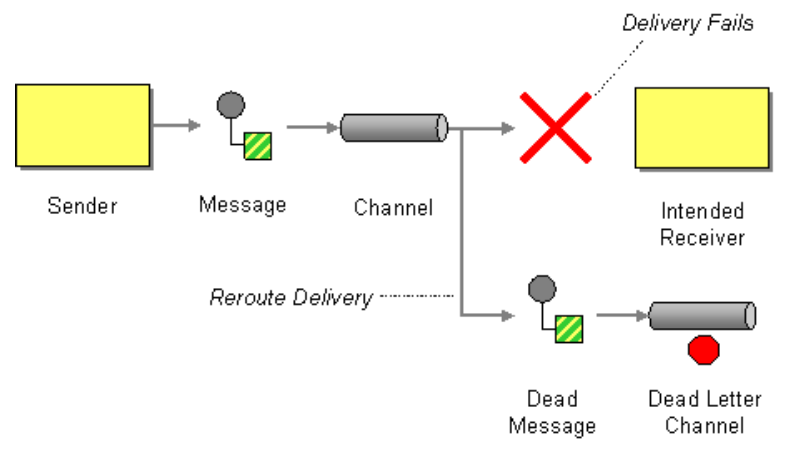
\includegraphics[width=0.5\textwidth]{deadletterchannelpattern}
  \caption{Dead Letter Channel Pattern}
\end{figure}

\subsection{Message Endpoint Pattern}
Connect an application to a messaging channel using a Message Endpoint, a client of the messaging system that the application can then use to send or receive messages.

\textbf{Key considerations:}
\begin{itemize}
  \item Number of consumer endpoints? Push vs. pull (be event-driven)?
  \item Behavior of consumers: competing? browse message or remove it from queue?
  \item Idempotency (i.e., resending identical request messages does not change state of receiving application)?
  \item transactional semantics (ACID properties, local/distributed 2PC)?
\end{itemize}

\begin{figure}[H]
  \center
  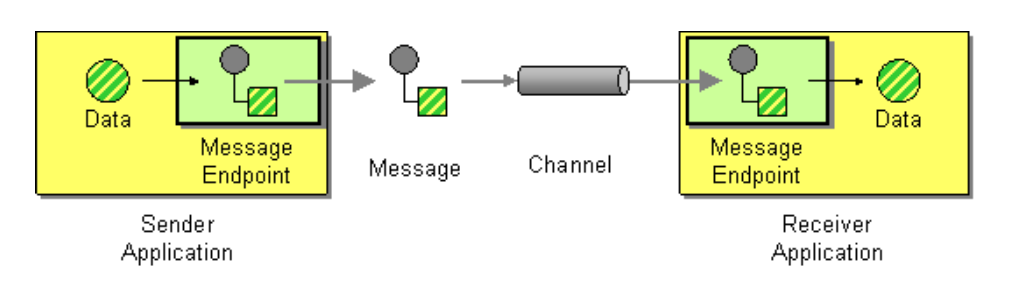
\includegraphics[width=0.75\textwidth]{messageendpoint}
  \caption{Message Endpoint Pattern}
\end{figure}

\subsubsection{Message Consumption: Competing Consumers}
Create multiple Competing Consumers on a single channel so that the consumers can process multiple messages concurrently. Competing Consumers are multiple consumers that are all created to receive messages from a single Point-to-Point Channel. When the channel delivers a message, any of the consumers could potentially receive it. The messaging system's implementation determines which consumer actually receives the message, but in effect the consumers compete with each other to be the receiver. Once a consumer receives a message, it can delegate to the rest of its application.

\begin{figure}[H]
  \center
  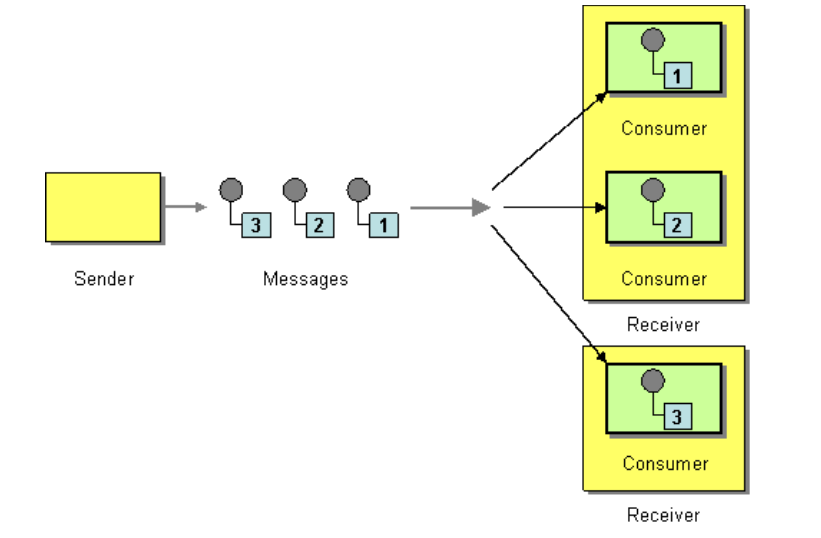
\includegraphics[width=0.5\textwidth]{competingconsumers}
  \caption{Competing Consumers}
\end{figure}

\subsubsection{Message Consumption: Selective Consumers}
Make the consumer a Selective Consumer, one that filters the messages delivered by its channel so that it only receives the ones that match its criteria.

\begin{figure}[H]
  \center
  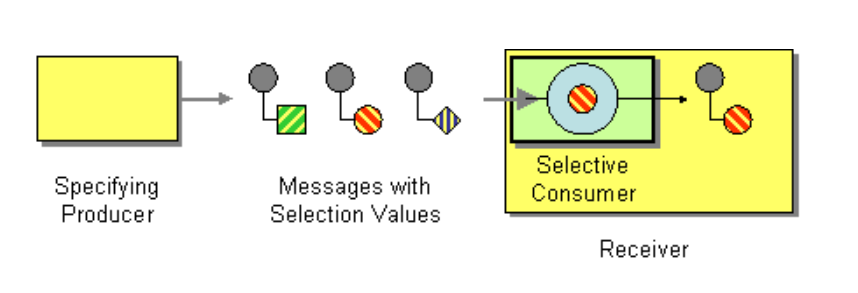
\includegraphics[width=0.5\textwidth]{selectiveconsumer}
  \caption{Selective Consumer}
\end{figure}

\subsubsection{Message Consumption: Polling Consumer}
The application can use a Polling Consumer, one that explicitly makes a call when it wants to receive a message. Also known as a synchronous receiver, because the receiver thread blocks until a message is received. We call it a Polling Consumer because the receiver polls for a message, processes it, then polls for another. As a convenience, messaging API’s usually provide a receive method that blocks until a message is delivered, in addition to methods like receiveNoWait() and Receive(0) that return immediately if no message is available. This difference is only apparent when the receiver is polling faster than messages are arriving.

\begin{figure}[H]
  \center
  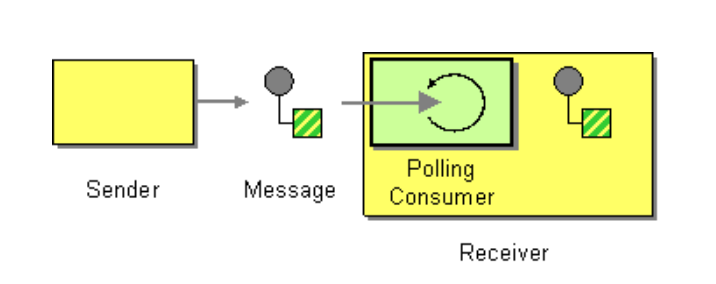
\includegraphics[width=0.5\textwidth]{pollingconsumer}
  \caption{Polling Consumer}
\end{figure}

\subsubsection{Event-Driven Consumer}
he application should use an Event-Driven Consumer, one that is automatically handed messages as they’re delivered on the channel. This is also known as an asynchronous receiver, because the receiver does not have a running thread until a callback thread delivers a message. We call it an Event-Driven Consumer because the receiver acts like the message delivery is an event that triggers the receiver into action.

\begin{figure}[H]
  \center
  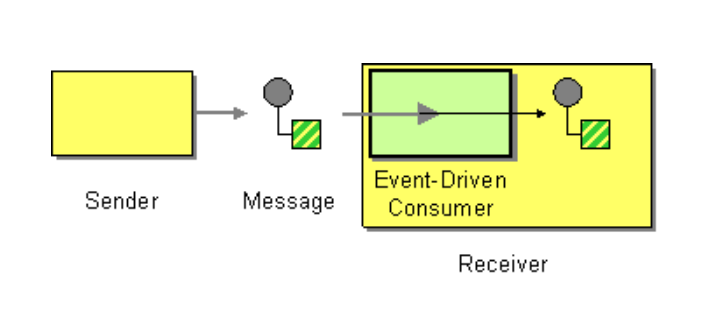
\includegraphics[width=0.5\textwidth]{eventdrivenconsumer}
  \caption{Event-Driven Consumer}
\end{figure}

\subsubsection{Transactional Client Pattern}
Use a Transactional Client – make the client’s session with the messaging system transactional so that the client can specify transaction boundaries. Both a sender and a receiver can be transactional. With a sender, the message isn’t “really” added to the channel until the sender commits the transaction. With a receiver, the message isn’t “really” removed from the channel until the receiver commits the transaction.

\begin{figure}[H]
  \center
  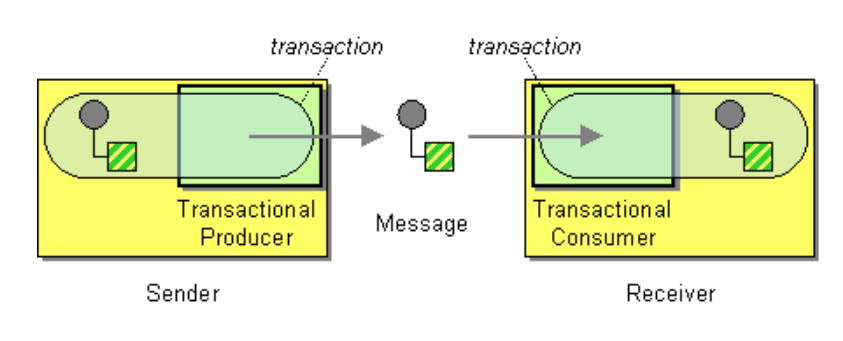
\includegraphics[width=0.5\textwidth]{transactionalclientpattern}
  \caption{Transactional Client Pattern}
\end{figure}

\pagebreak

\subsection{Message Routing Patterns}

\subsubsection{Message Router Pattern}
Insert a special filter, a Message Router, which consumes a Message from one Message Channel and republishes it to a different Message Channel depending on a set of conditions. The Message Router differs from the most basic notion of Pipes and Filters in that it connects to multiple output channels. Thanks to the Pipes and Filters architecture the components surrounding the Message Router are completely unaware of the existence of a Message Router. A key property of the Message Router is that it does not modify the message contents. It only concerns itself with the destination of the message.

\begin{figure}[H]
  \center
  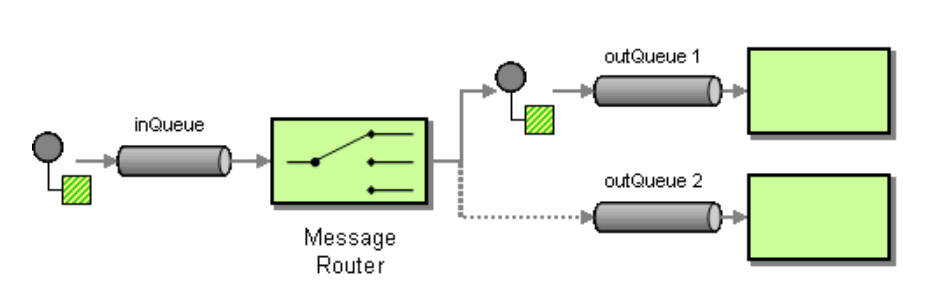
\includegraphics[width=0.65\textwidth]{messageroutingpattern}
  \caption{Message Router Pattern}
\end{figure}

\subsubsection{Content-Based Router Pattern}
Use a Content-Based Router to route each message to the correct recipient based on message content. The Content-Based Router examines the message content and routes the message onto a different channel based on data contained in the message. When implementing a Content-Based Router, special caution should be taken to make the routing function easy to maintain as the router can become a point of frequent maintenance.

\begin{figure}[H]
  \center
  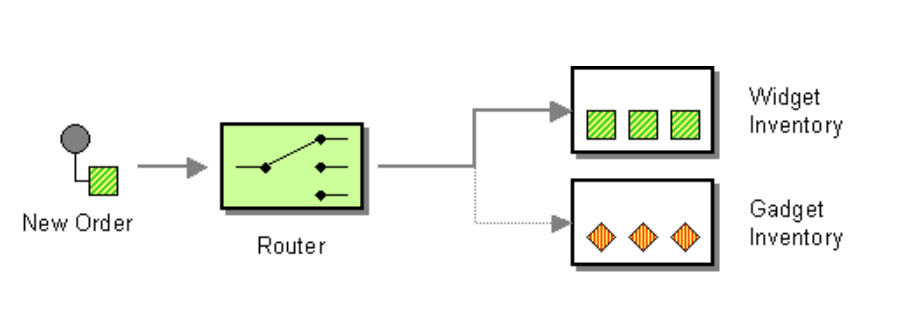
\includegraphics[width=0.5\textwidth]{contentbasedrouterpattern}
  \caption{Content Based Router Pattern}
\end{figure}

\subsubsection{Recipient List Pattern}
Define a channel for each recipient. Then use a Recipient List to inspect an incoming message, determine the list of desired recipients, and forward the message to all channels associated with the recipients in the list. The logic embedded in a Recipient List can be pictured as two separate parts even though the implementation is often coupled together. The first part computes a list of recipients. The second part simply traverses the list and sends a copy of the received message to each recipient.

\begin{figure}[H]
  \center
  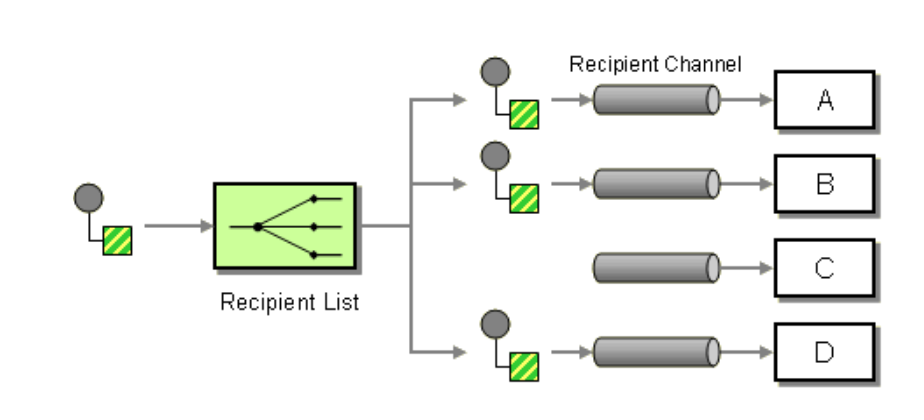
\includegraphics[width=0.65\textwidth]{recipientlistpattern}
  \caption{Recipient List Pattern}
\end{figure}

\subsubsection{Splittern Pattern}
Use a Splitter to break out the composite message into a series of individual messages, each containing data related to one item. Use a Splitter that consumes one message containing a list of repeating elements, each of which can be processed individually.

\begin{figure}[H]
  \center
  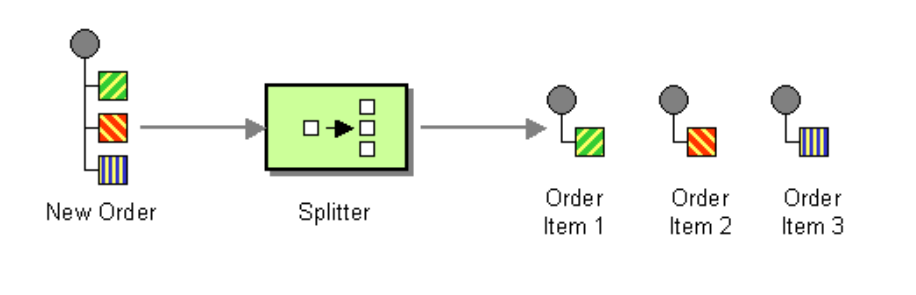
\includegraphics[width=0.65\textwidth]{splitterpattern}
  \caption{Splitter Pattern}
\end{figure}

\subsubsection{Aggregator Pattern}
Use a stateful filter, an Aggregator, to collect and store individual messages until a complete set of related messages has been received. Then, the Aggregator publishes a single message distilled from the individual messages. The Aggregator is a special Filter that receives a stream of messages and identifies messages that are correlated. Once a complete set of messages has been received the Aggregator collects information from each correlated message and publishes a single, aggregated message to the output channel for further processing.

\begin{figure}[H]
  \center
  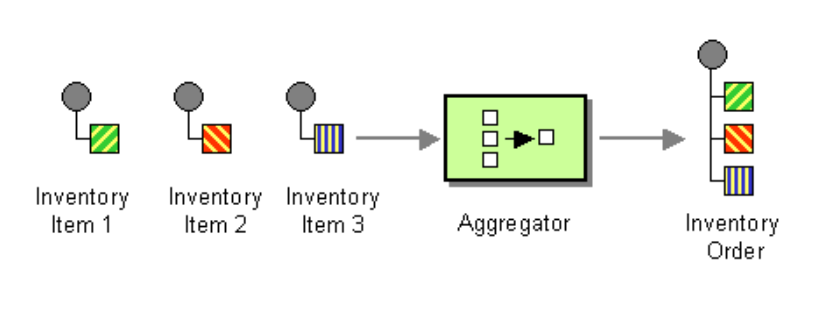
\includegraphics[width=0.5\textwidth]{aggregatorpattern}
  \caption{Aggregator Pattern}
\end{figure}

\pagebreak

\subsection{Message Transformation Patterns}
The EIP book describes six universal message transformation patterns. These patterns are highly applicable to Enterprise Application Integration (EAI).

\subsubsection{Message Translation Pattern}
Use a special filter, a Message Translator, between other filters or applications to translate one data format into another. The Message Translator is the messaging equivalent of the general Adapter design pattern. An adapter converts the interface of a component into a another interface so it can be used in a different context.

\begin{figure}[H]
  \center
  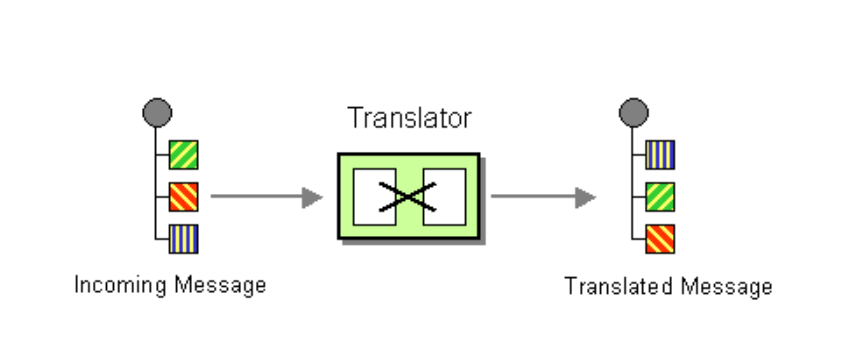
\includegraphics[width=0.5\textwidth]{messagetranslatorpattern}
  \caption{Message Translator Pattern}
\end{figure}

\subsubsection{Content Filter Pattern}
Use a Content Filter to remove unimportant data items from a message leaving only important items. The Content Filter does not necessarily just remove data elements. A Content Filter is also useful to simplify the structure of the message. Often times, messages are represented as tree structures. Many messages originating from external systems or packaged applications contain many levels of nested, repeating groups because they are modeled after generic, normalized database structures.

\begin{figure}[H]
  \center
  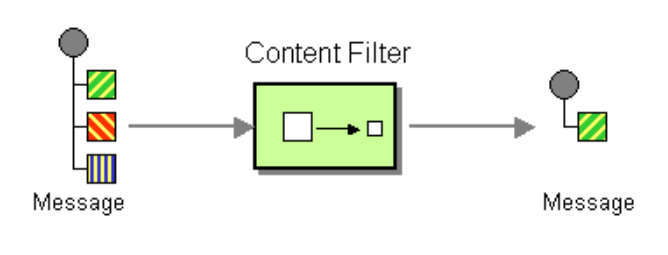
\includegraphics[width=0.45\textwidth]{contentfilter}
  \caption{Content Filter}
\end{figure}

\subsubsection{Content Enricher Pattern}
Use a specialized transformer, a Content Enricher (a.k.a. Data Enricher), to access an external data source in order to augment a message with missing information. The Content Enricher uses information inside the incoming message (e.g. key fields) to retrieve data from an external source. After the Content Enricher has retrieved the required data from the resource, it appends the data to the message.

\begin{figure}[H]
  \center
  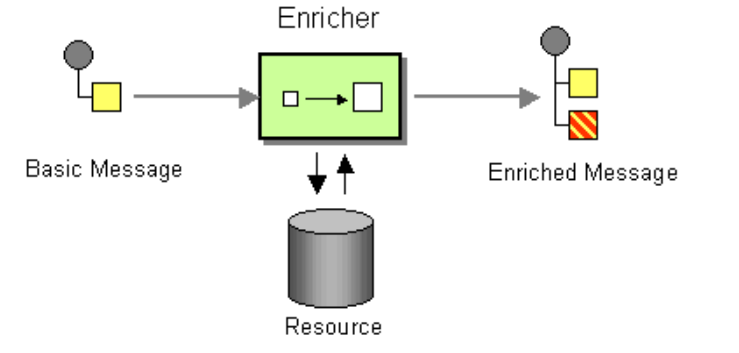
\includegraphics[width=0.5\textwidth]{conentenricherpattern}
  \caption{Content Enricher Pattern}
\end{figure}

